\documentclass[11pt,a4paper]{article}

% =============================================================================
% PACKAGES & DOCUMENT SETUP
% =============================================================================
\usepackage[utf8]{inputenc}
\usepackage[margin=1in]{geometry}
\usepackage{amsmath, amssymb, amsthm}
\usepackage{graphicx}
\usepackage{xcolor}
\usepackage{hyperref}
\usepackage{fancyhdr}
\usepackage{listings}
\usepackage{booktabs}
\usepackage{tabularx}
\usepackage{tikz}
\usepackage{float}
\usetikzlibrary{shapes.geometric, arrows.meta, positioning, calc, fit, backgrounds, shadows}

% =============================================================================
% SPEZI COLOR PALETTE
% =============================================================================
\definecolor{primary}{RGB}{224, 86, 36}      % Spezi Vibrant Sunburst Orange
\definecolor{secondary}{RGB}{26, 31, 76}     % Paulaner Midnight Navy
\definecolor{accent}{RGB}{245, 158, 11}      % Spezi Citrus Gold
\definecolor{darkbg}{RGB}{255, 251, 245}     % Cream White Background
\definecolor{codebg}{RGB}{255, 247, 237}     % Soft Light Orange Tint for Code
\definecolor{codecomment}{RGB}{148, 87, 85}  % Muted Burgundy Comments
\definecolor{codestring}{RGB}{180, 83, 9}    % Spezi Amber Strings
\definecolor{codekeyword}{RGB}{157, 23, 77}  % Deep Spezi Magenta Keywords

% Hyperlink Configuration
\hypersetup{
    colorlinks=true,
    linkcolor=primary,
    citecolor=secondary,
    urlcolor=primary,
    pdftitle={Project Accountability Documentation},
    pdfauthor={Guillermo Ramos Santos, Itamar Fink},
    pdfsubject={Final Cryptography Project - Group E}
}

% Header and Footer Setup
\pagestyle{fancy}
\fancyhf{}
\setlength{\headheight}{14pt}
\rhead{\textcolor{primary}{\small Project Accountability --- Technical Documentation}}
\lhead{\textcolor{secondary}{\small Group E}}
\rfoot{\thepage}
\lfoot{\textcolor{secondary}{\small Cryptography \& System Security}}
\renewcommand{\headrulewidth}{0.4pt}
\renewcommand{\footrulewidth}{0.4pt}

% Code Listing Configuration
\lstset{
    language=C++,
    backgroundcolor=\color{codebg},
    basicstyle=\ttfamily\footnotesize,
    keywordstyle=\color{codekeyword}\bfseries,
    stringstyle=\color{codestring},
    commentstyle=\color{codecomment}\itshape,
    numbers=left,
    numberstyle=\tiny\color{codecomment},
    stepnumber=1,
    numbersep=8pt,
    showstringspaces=false,
    breaklines=true,
    frame=single,
    rulecolor=\color{primary!40},
    tabsize=2,
    captionpos=b
}

% Callout Box Styling
% Keep callout boxes dependency-free so the document builds with a basic TeX
% installation as well as a full TeX Live installation.
\newenvironment{infobox}[1][]
  {\begin{center}\begin{minipage}{0.88\textwidth}\noindent\textbf{#1}\par\smallskip\hrule\smallskip}
  {\end{minipage}\end{center}}
\newenvironment{warningbox}[1][]
  {\begin{center}\begin{minipage}{0.88\textwidth}\noindent\textcolor{codekeyword}{\textbf{#1}}\par\smallskip\hrule\smallskip}
  {\end{minipage}\end{center}}

% =============================================================================
% DOCUMENT START
% =============================================================================
\begin{document}

% -----------------------------------------------------------------------------
% COVER PAGE
% -----------------------------------------------------------------------------
\begin{titlepage}
	\centering
	\vspace*{1cm}

	{\Huge \bfseries \color{primary} Project Accountability} \\[0.4cm]
	{\Large \color{secondary} Secure Group Messaging with Auditable Threshold Key-Escrow} \\[1.5cm]

	\rule{\linewidth}{0.5mm} \\[1.5cm]

	\begin{minipage}{0.48\textwidth}
		\begin{flushleft} \large
			\textbf{Authors:}\\[0.2cm]
			Guillermo \textsc{Ramos Santos} \\
			Itamar \textsc{Fink} \\
			\textit{(Group E)}
		\end{flushleft}
	\end{minipage}
	~
	\begin{minipage}{0.48\textwidth}
		\begin{flushright} \large
			\textbf{Course / Context:}\\[0.2cm]
			Praktikum Cryptography \\
			Final Project Documentation \\
			\today
		\end{flushright}
	\end{minipage}

	\vfill

	\begin{infobox}[Summary]
		\small
		\textit{Project Accountability} is an end-to-end group-messaging prototype with a shared group secret and threshold key escrow. The platform integrates:
		\begin{itemize}
			\item \textbf{Shared-Secret Group Chat:} One RSA-encrypted copy of a randomly generated group secret per member; AES-CBC, HMAC, and per-message RSA-PSS signatures protect normal records.
			\item \textbf{Certified Setup:} The server certifies each user's signing and encryption RSA public keys, and the creator signs the complete group-creation request.
			\item \textbf{Threshold Key Escrow:} A $(t,n)$ Feldman Distributed Key Generation (DKG) and ElGamal threshold-decryption scheme with Chaum-Pedersen-style partial-decryption proofs. Recovery needs the configured threshold of cooperating escrows.
			\item \textbf{Interactive Terminal Interface:} A responsive, thread-safe Terminal UI (FTXUI) supporting background polling, diff rendering, and interactive group administration.
		\end{itemize}
	\end{infobox}

	\vfill
	{\small Repository: Group-E-Crypto-Final}
\end{titlepage}

\newpage
\pagenumbering{roman}

% -----------------------------------------------------------------------------
% TABLE OF CONTENTS & LISTS
% -----------------------------------------------------------------------------
\tableofcontents
\newpage
\listoffigures
\listoftables
\newpage

\pagenumbering{arabic}

% =============================================================================
% 1. INTRODUCTION & SYSTEM OBJECTIVES
% =============================================================================
\section{Introduction \& System Objectives}
\label{sec:introduction}

Modern messaging applications prioritize absolute forward secrecy and privacy, often preventing legitimate, court-ordered oversight or regulatory auditing in high-stake governance settings. \textbf{Project Accountability} reconciles privacy with legal auditability through split-control key escrow.

\subsection{Key Goals \& Architectural Guarantees}
\begin{enumerate}
	\item \textbf{Group Chat Confidentiality:} A creator samples one shared group secret $m=G^k \in \mathbb{Z}_p^*$ and creates one RSA envelope for every member. Messages use AES-CBC and HMAC keys derived from $m$.
	\item \textbf{Authenticated Setup and Messages:} The creator signs the full group-creation request, and every normal encrypted message record is RSA-PSS signed with its sender's separate signing key. The shared HMAC still authenticates possession of the group secret; the RSA signature supplies individual authorship.
	\item \textbf{Auditable Threshold Escrow:} Per-group escrow envelopes store ElGamal ciphertexts of group secrets under a collective public key $pk = G^s$. The corresponding secret key $s$ is distributed across $n$ independent Escrow Trustees using a $(t,n)$ Distributed Key Generation (DKG) scheme. No single party (including the central server) holds $s$.
	\item \textbf{Honest-but-Curious Server Blindness:} The central relay coordinates messages, user authentication, and DKG rounds, and stores ciphertexts and metadata. It does not receive a group secret or an escrow private share.
	\item \textbf{Robust Terminal UI:} An FTXUI-based client frontend providing differential message history rendering, thread-safe state management, and real-time network status feedback.
\end{enumerate}

% =============================================================================
% 2. SYSTEM ARCHITECTURE & CLASS DIAGRAM
% =============================================================================
\section{System Architecture \& Component Design}
\label{sec:architecture}

The system is composed of three primary network entities: the \textbf{Auth Server}, \textbf{User Clients}, and \textbf{Escrow Nodes}.

\subsection{Class \& Component Hierarchy}

Below is the conceptual class diagram illustrating the key C++ modules, their responsibilities, and structural relationships. The diagram is formatted with spacious padding to prevent overlapping elements.

\begin{figure}[H]
	\centering
	\resizebox{0.88\textwidth}{!}{%
	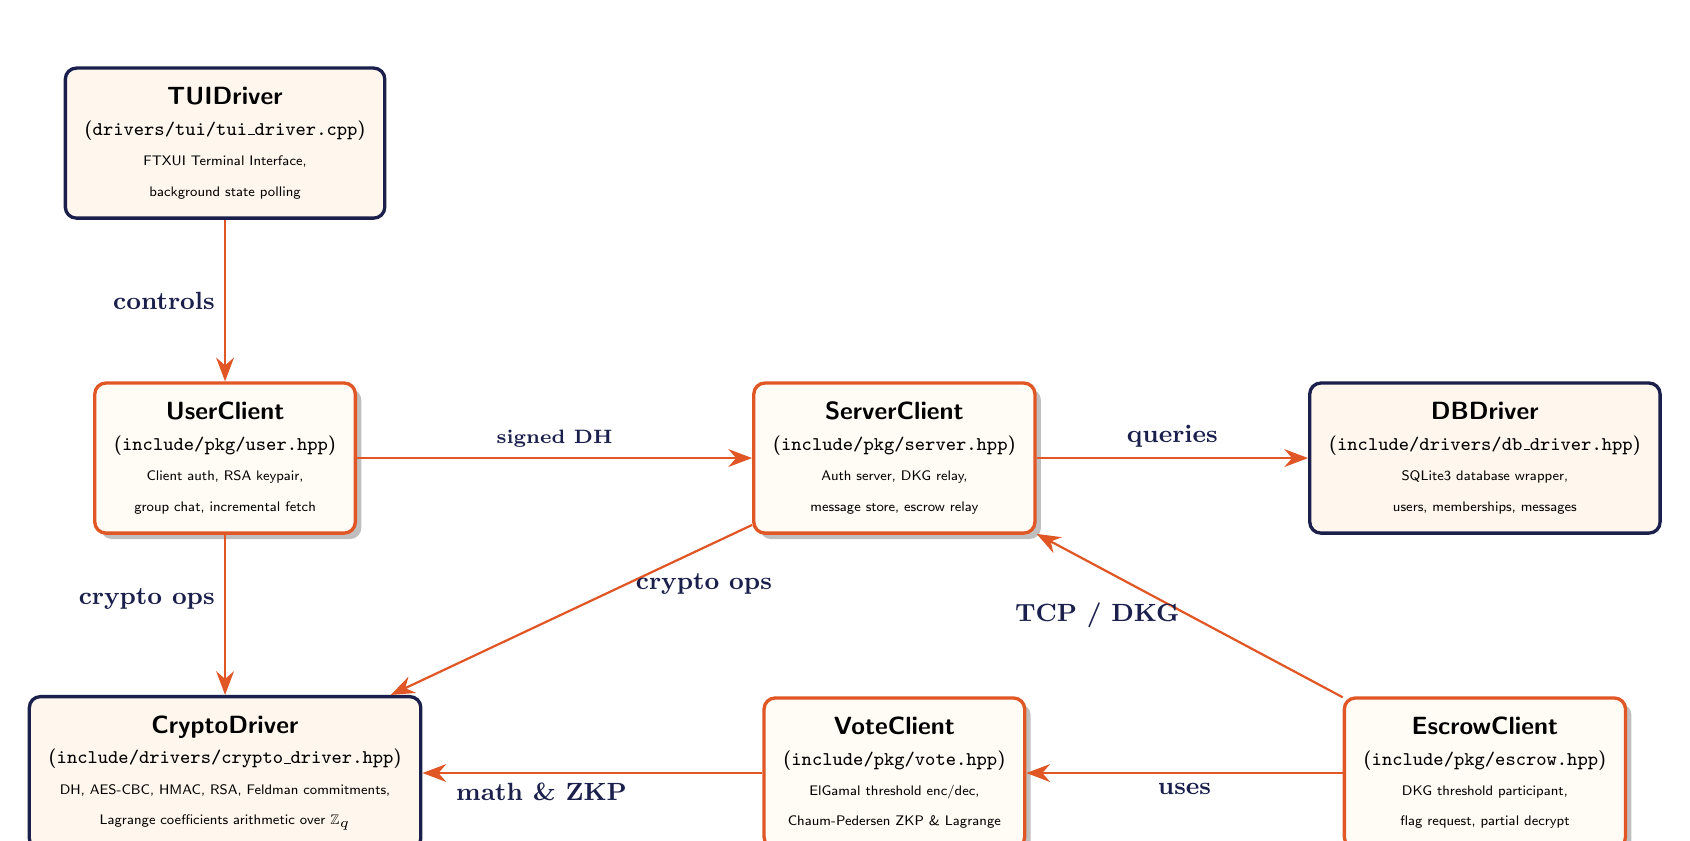
\begin{tikzpicture}[
		box/.style={draw=primary, fill=darkbg, rounded corners=4pt, font=\sffamily\small, align=center, inner sep=7pt, minimum width=3.2cm, minimum height=1.3cm, very thick, drop shadow},
		driver/.style={draw=secondary, fill=codebg, rounded corners=4pt, font=\sffamily\small, align=center, inner sep=7pt, minimum width=3.2cm, minimum height=1.3cm, very thick},
		arrow/.style={-{Stealth[scale=1.3]}, thick, draw=primary}
		]

		% Top Row: UI & Network Entities
		\node[driver] (tui) at (-7, 4) {\textbf{TUIDriver}\\ \scriptsize (\texttt{drivers/tui/tui\_driver.cpp})\\ \tiny FTXUI Terminal Interface, \\ \tiny background state polling};

		\node[box] (user) at (-7, 0) {\textbf{UserClient}\\ \scriptsize (\texttt{include/pkg/user.hpp})\\ \tiny Client auth, RSA keypair, \\ \tiny group chat, incremental fetch};

		\node[box] (server) at (1.5, 0) {\textbf{ServerClient}\\ \scriptsize (\texttt{include/pkg/server.hpp})\\ \tiny Auth server, DKG relay, \\ \tiny message store, escrow relay};

		\node[box] (escrow) at (9, -4) {\textbf{EscrowClient}\\ \scriptsize (\texttt{include/pkg/escrow.hpp})\\ \tiny DKG threshold participant, \\ \tiny flag request, partial decrypt};

		% Middle Row: Data Persistence & Escrow Vote Logic
		\node[driver] (db) at (9, 0) {\textbf{DBDriver}\\ \scriptsize (\texttt{include/drivers/db\_driver.hpp})\\ \tiny SQLite3 database wrapper, \\ \tiny users, memberships, messages};

		\node[box] (vote) at (1.5, -4) {\textbf{VoteClient}\\ \scriptsize (\texttt{include/pkg/vote.hpp})\\ \tiny ElGamal threshold enc/dec, \\ \tiny Chaum-Pedersen ZKP \& Lagrange};

		% Bottom Row: Cryptographic Primitives Foundation
		\node[driver] (crypto) at (-7, -4) {\textbf{CryptoDriver}\\ \scriptsize (\texttt{include/drivers/crypto\_driver.hpp})\\ \tiny DH, AES-CBC, HMAC, RSA, Feldman commitments, \\ \tiny Lagrange coefficients arithmetic over $\mathbb{Z}_q$};

		% Connections & Relationships
		\draw[arrow] (tui) -- node[left, font=\small\bfseries, color=secondary]{controls} (user);
		\draw[arrow] (user) -- node[above, font=\scriptsize\bfseries, color=secondary]{signed DH} (server);
		\draw[arrow] (escrow) -- node[left, font=\small\bfseries, color=secondary]{TCP / DKG} (server);
		\draw[arrow] (server) -- node[above, font=\small\bfseries, color=secondary]{queries} (db);
		\draw[arrow] (escrow) -- node[below, font=\small\bfseries, color=secondary]{uses} (vote);

		\draw[arrow] (user) -- node[left, font=\small\bfseries, color=secondary, pos=0.4]{crypto ops} (crypto);
		\draw[arrow] (server) -- node[right, font=\small\bfseries, color=secondary, pos=0.35]{crypto ops} (crypto);
		\draw[arrow] (vote) -- node[below, font=\small\bfseries, color=secondary, pos=0.65]{math \& ZKP} (crypto);

	\end{tikzpicture}%
	}
	\caption{System Architecture \& Class Dependencies Diagram}
	\label{fig:class_diagram}
\end{figure}

\subsection{Summary of Key Modules}
\begin{table}[H]
	\centering
	\small
	\renewcommand{\arraystretch}{1.4}
	\begin{tabularx}{\textwidth}{l l X}
		\toprule
		\textbf{Module Class} & \textbf{Header / Source}                     & \textbf{Primary Responsibilities}                                                                                                 \\
		\midrule
		\texttt{ServerClient} & \texttt{include/pkg/server.hpp}              & User registration/login, DKG orchestration, signed-message storage/verification, and blinded escrow response relaying.            \\ \hline
		\texttt{UserClient}   & \texttt{include/pkg/user.hpp}                & Client auth, two RSA key pairs, group-secret envelopes, signed-message verification, certificate cache, and incremental fetch.   \\ \hline
		\texttt{EscrowClient} & \texttt{include/pkg/escrow.hpp}              & Threshold share holder, DKG participant, flag initiator, partial decryptor, and recovered-message signature verifier.             \\ \hline
		\texttt{CryptoDriver} & \texttt{include/drivers/crypto\_driver.hpp}  & Low-level cryptographic primitives (CryptoPP wrappers), Feldman commitments, Lagrange coefficient arithmetic over $\mathbb{Z}_q$. \\ \hline
		\texttt{VoteClient}   & \texttt{include/pkg/vote.hpp}                & ElGamal threshold encryption, Chaum-Pedersen ZKP generation/verification, Lagrange partial share combination.                     \\ \hline
		\texttt{DBDriver}     & \texttt{include/drivers/db\_driver.hpp}      & SQLite3 database wrapper managing user accounts, group memberships, and persistent signed-message logs.                           \\ \hline
		\texttt{TUIDriver}    & \texttt{include/drivers/tui/tui\_driver.hpp} & FTXUI interface, periodic group polling, flicker-free differential message rendering.                                             \\
		\bottomrule
	\end{tabularx}
	\caption{Module Breakdown and Source Locations}
	\label{tab:modules}
\end{table}

% =============================================================================
% 3. IMPLEMENTED PROTOCOL FLOW
% =============================================================================
\section{Implemented Protocol Flow}
\label{sec:flow}

\subsection{Configuration and trust boundary}

The threshold values are compile-time program constants, \texttt{THRESHOLD\_T} and \texttt{THRESHOLD\_N}, in \texttt{include-shared/constants.hpp}. They are not chosen by a user when a group is created. Changing either value requires a matching update to the authorized escrow IDs and per-escrow server-authentication secrets in \texttt{include-shared/escrow\_security.hpp}, plus matching escrow configuration files.

\begin{infobox}[Current checkout]
The checked-in configuration uses $t=3$, $n=5$, the authorized escrow IDs \texttt{1} through \texttt{5}, and five matching escrow configuration files. The description below remains parametric: a changed threshold is safe only when the roster, per-escrow secrets, and configuration files are updated together.
\end{infobox}

The server is intended to be honest-but-curious. It sees user IDs, group IDs, group membership, message IDs, timestamps/order, IVs, ciphertext lengths, ciphertexts, and MACs. It is not given a user's RSA private key, a group secret, the escrow mesh secret, or an escrow's group-specific threshold share. The escrow mesh secret is assumed to be provisioned independently to the fixed escrow set.

\subsection{User registration and login}

The relevant code is \texttt{UserClient::HandleServerKeyExchange} and \texttt{DoLoginOrRegister} in \texttt{src/pkg/user.cxx}, and \texttt{ServerClient::HandleKeyExchange}, \texttt{HandleRegister}, and \texttt{HandleLogin} in \texttt{src/pkg/server.cxx}.

\begin{enumerate}
	\item The client sends an ephemeral DH public value $X$. The server generates its own ephemeral DH value $Y$, echoes $X$, and returns an RSA-PSS/SHA-256 signature over $Y\mathbin\Vert X$.
	\item The client verifies that signature with the server verification key configured locally and checks the echoed value. Both sides derive a fresh DH secret. \texttt{CryptoDriver} derives an AES key with HKDF/SHA-256 and fixed salt \texttt{salt0000}, and a separate HMAC key with fixed salt \texttt{salt0001}.
	\item Subsequent connection messages use AES-CBC with a fresh IV and encrypt-then-HMAC. The transport HMAC covers \texttt{IV || ciphertext}, and the receiver verifies it before CBC decryption. This is custom TCP cryptography, not TLS.
	\item During registration the server supplies a fresh 16-byte salt. The client sends the binary SHA-256 value $H(\textit{password}\mathbin\Vert\textit{salt})$ through the authenticated channel; the server stores that hash and salt. Login repeats that comparison. There is no pepper, PRG challenge, TOTP, or other second factor.
	\item After a successful registration, the client generates two independent 3072-bit RSA key pairs: one signing pair and one encryption pair. The server signs the account ID, signing public key, and encryption public key to form a certificate. The client saves the certificate and both private keys locally.
\end{enumerate}

The signed DH exchange authenticates the configured server to a client. User authentication itself is password-based. SHA-256 is a fast hash, rather than a password-hardening KDF, so a database compromise permits offline password guessing.

\subsection{Per-group DKG and group creation}

\texttt{UserClient::HandleGroupCreate} first calls \texttt{EnsureGroupDKG}. \texttt{ServerClient::StartGroupDKG} reserves the group ID for the authenticated creator; escrows then explicitly enter \texttt{keygen <group-id>}. The server accepts a key-generation attempt only for the active group ID, and every escrow verifies that the server's DKG start message names the group ID it entered.

Each escrow $i$ selects a degree-$(t-1)$ polynomial $f_i$, sends Feldman commitments $G^{c_{i,j}}$, and sends each other escrow $j$ its share $f_i(j)$ under the escrow-only AES-CBC/HMAC mesh. Recipient $j$ authenticates and decrypts the share, verifies it against the commitments, and stores its final share $z_j=\sum_i f_i(j)\pmod Q$ and public verification share $G^{z_j}$ in files whose names are derived from the group ID. The server persists the collective DKG public key $pk=G^{\sum_i c_{i,0}}$ and reported partial public keys only after all $n$ escrows complete.

Once the DKG is complete, the creator performs the following setup in \texttt{UserClient::HandleGroupCreate}:

\begin{enumerate}
	\item It inserts itself into the member set, samples $k\leftarrow\mathbb{Z}_Q^*$, and computes the shared group secret $m=G^k\bmod P$.
	\item For each member it fetches and verifies that member's server-signed certificate, then uses the member's \emph{encryption} RSA public key $(n_j,e_j)$ to form one envelope $C_j=m^{e_j}\bmod n_j$. The corresponding private operation gives $m=C_j^{d_j}\bmod n_j$.
	\item It encrypts the same $m$ under the DKG public key using ElGamal: $a=G^r\bmod P$ and $b=m\,pk^r\bmod P$. This is the escrow envelope.
	\item It serializes the group ID, member list, member envelopes, and escrow envelope, then signs those bytes with the creator's RSA \emph{signing} private key. The signature field is empty while the signed bytes are serialized.
	\item The server verifies that the DKG belongs to the authenticated creator, every member is registered, envelopes name exactly the members, and the creator signature verifies under the creator's certified signing public key. It stores the opaque envelopes and membership in SQLite.
\end{enumerate}

There is one shared group secret and one member envelope per member; there are no sender keys. The creation signature authenticates the setup request only. The server cannot inspect a raw RSA envelope to prove that it contains the same secret as the ElGamal escrow ciphertext, so consistency of those values relies on the trusted creator.

\subsection{Normal group messaging}

\texttt{HandleGroupSend}, \texttt{HandleGroupFetch}, and \texttt{FetchGroupMessagesStructured} in \texttt{src/pkg/user.cxx} implement normal messaging. A member fetches its own envelope, applies its RSA encryption private operation, and derives group AES and HMAC keys from the recovered $m$ using the same two HKDF calls. To send plaintext $M$, it creates a fresh CBC IV and ciphertext $C$, then computes
\[
\tau=\operatorname{HMAC}_{K_G^{\mathrm{HMAC}}}(\textit{group\_id}\mathbin\Vert\textit{sender\_id}\mathbin\Vert IV\mathbin\Vert C).
\]
It then calls \texttt{group\_message\_signature\_input} in \texttt{src-shared/messages.cxx}. That function length-prefixes the domain label \texttt{group-message-signature-v1}, group ID, authenticated sender ID, IV, ciphertext, and $\tau$. The client uses its RSA signing private key to produce an RSA-PSS/SHA-256 signature $\sigma$ over those canonical bytes.

The send request is protected again by the client/server transport channel. There is no client-supplied sender field: the server takes the authenticated session user ID, verifies $\sigma$ against that user's stored server-certified signing public key, and stores $(\mathit{sender\_id},IV,C,\tau,\sigma)$. A recipient first verifies the inexpensive shared HMAC, then fetches and caches the sender's certificate by server endpoint and user ID, verifies the server's certificate signature, verifies $\sigma$, and only then CBC-decrypts $C$.

The UI maintains an in-memory cursor and cache, and asks for messages whose database ID is larger than its last cursor. It therefore transfers only newer records. Despite server support for a persistent request loop, the current \texttt{FetchGroupState} implementation opens, authenticates, fetches, and closes a new TCP connection for every poll.

All members know the same group HMAC key, so a valid HMAC alone only says that a holder of the group secret produced the record. The RSA-PSS signature binds that same encrypted record to the sender's certified signing key and prevents one group member from creating a valid record attributed to another. It does not prevent a server or group member from replaying an unchanged, valid record; there is no signed per-sender counter or recipient replay cache.

\subsection{Escrow recovery}

An escrow starts recovery with \texttt{flag <group-id>} in \texttt{EscrowClient::HandleFlag}; other escrows invoke \texttt{decrypt}. The requesting escrow sends a fresh DH public value $X_R$, a mesh-key HMAC binding its ID, group ID, and $X_R$, and a separate server-authentication HMAC. Responding escrows verify the mesh HMAC before they load only their group-specific share and public verification key.

A responder computes $d_i=a^{z_i}\bmod P$ and its partial-decryption proof. It creates a fresh DH key pair, derives wrapping keys from its DH secret with the requester, AES-CBC encrypts the partial/proof, and HMACs a context containing the responder ID, group ID, both DH public values, IV, and ciphertext. The server relays this opaque response. The requester contributes its own partial, decrypts and verifies each response and proof, then combines its own partial plus at least $t-1$ responder partials with Lagrange interpolation. The bundle also contains each stored signature and one server-signed certificate per distinct sender. After recovering $m$, the requester verifies each certificate with its configured server public key, verifies the group HMAC and the sender's RSA-PSS signature, then decrypts locally. The server never receives the recovered secret or plaintext.

% =============================================================================
% 4. MATHEMATICAL & CRYPTOGRAPHIC FOUNDATIONS
% =============================================================================
\section{Cryptographic Protocols \& Mathematics}
\label{sec:crypto_math}

\subsection{Discrete Logarithm Group Settings}
The threshold and ElGamal schemes operate over the fixed RFC~5114-style multiplicative subgroup parameters in \texttt{include-shared/constants.hpp}.  The implementation requires that $G$ has order $Q$ modulo $P$; it does not assume or use $P=2Q+1$:
\[
	\text{Group Parameters: } (P, Q, G) \quad \text{where } G \in \mathbb{Z}_P^* \text{ has order } Q.
\]

\subsection{Feldman Distributed Key Generation (DKG)}
To establish a per-group escrow public key $pk = G^s$ without any single entity knowing $s$:
\begin{enumerate}
	\item Each escrow node $i \in \{1, \dots, n\}$ selects a secret polynomial $f_i(x) \in \mathbb{Z}_q[x]$ of degree $t-1$:
	      \[
		      f_i(x) = c_{i,0} + c_{i,1} x + \dots + c_{i,t-1} x^{t-1} \pmod q
	      \]
	\item Node $i$ broadcasts Feldman commitments:
	      \[
		      C_{i,j} = G^{c_{i,j}} \bmod P \quad \text{for } j \in \{0, \dots, t-1\}
	      \]
	\item Node $i$ privately distributes share $f_i(j)$ to node $j$ in an AES-CBC/HMAC envelope protected by the pre-provisioned escrow-only mesh key. The HMAC binds the group ID, sender ID, recipient ID, IV, and ciphertext; the server relays the opaque envelope.
	\item Each node $j$ verifies received share $s_{i \to j}$ against published commitments:
	      \[
		      G^{s_{i \to j}} \stackrel{?}{=} \prod_{k=0}^{t-1} \left(C_{i,k}\right)^{j^k} \bmod P
	      \]
	\item Combined share of escrow $j$ is $z_j = \sum_{i=1}^n f_i(j) \bmod q$. The total secret is $s = \sum_{i=1}^n c_{i,0} \bmod q$, and public key is $pk = G^s \bmod P$.
\end{enumerate}

\subsection{ElGamal Threshold Encryption \& Partial Decryption ZKP}
When a group is initialized, the creator generates a random exponent $k \xleftarrow{R} \mathbb{Z}_q^*$ and computes $m = G^k \bmod P$. The creator then wraps $m$ using ElGamal threshold encryption:
\[
	a = G^r \bmod P, \quad b = m \cdot pk^r \bmod P \quad (r \xleftarrow{R} \mathbb{Z}_q^*)
\]
Group members derive symmetric AES-CBC and HMAC keys from $m$. To decrypt via threshold escrow, each escrow node $i$ must contribute its partial decryption share $d_i$. Formally, each node $i$ possesses a secret share $z_i \in \mathbb{Z}_q$ (derived during Feldman VSS) and a corresponding public key share $pk_i = G^{z_i} \bmod P$. Node $i$ computes its partial decryption $d_i$ by exponentiating ciphertext component $a$ with its private share $z_i$:
\[
	d_i = a^{z_i} \bmod P
\]

\paragraph{Mathematical Relationship between $d_i$ and $pk_i$:}
Notice the key structural symmetry between the node's public key share $pk_i$ and its partial decryption share $d_i$:
\[
	pk_i = G^{z_i} \bmod P \quad (\text{base } G), \qquad d_i = a^{z_i} \bmod P \quad (\text{base } a)
\]
Both $pk_i$ and $d_i$ are modular exponentiations sharing the \textbf{exact same secret exponent} $z_i$, evaluated over different bases (the generator $G$ versus the ciphertext component $a = G^r \bmod P$). Consequently, their discrete logarithms satisfy:
\[
	\log_G(pk_i) = z_i = \log_a(d_i)
\]
To prove that node $i$ correctly computed $d_i$ using its authentic secret share $z_i$ without disclosing $z_i$, node $i$ produces a \textbf{Chaum-Pedersen Zero-Knowledge Proof} $(u, v, s)$ asserting $\log_G(pk_i) = \log_a(d_i)$:
\begin{align*}
	u      & = G^\omega \bmod P, \quad v = a^\omega \bmod P \quad (\omega \xleftarrow{R} \mathbb{Z}_q) \\
	\sigma & = H(pk_i \,||\, a \,||\, d_i \,||\, u \,||\, v) \bmod q                                   \\
	s      & = (\omega + z_i \cdot \sigma) \bmod q
\end{align*}

\subsection{Intuition \& Mathematics of Threshold Secret Sharing via Lagrange Interpolation}
\label{subsec:lagrange_intuition}

To understand how $(t, n)$ threshold decryption works without revealing intermediate secret keys, we examine the fundamental geometric principle of polynomial interpolation.

\subsubsection{Geometric Principle: The 2-Point Line Axiom}
In Euclidean geometry, \textbf{a straight line (degree-1 polynomial) is uniquely determined by 2 points}. 
\begin{itemize}
	\item \textbf{1 Point is Insufficient (Zero Information):} If an attacker or single escrow node possesses only 1 share $(x_1, y_1)$, there are \textbf{infinitely many straight lines} passing through $(x_1, y_1)$. Every possible secret $s' \in \mathbb{Z}_q$ corresponds to a valid candidate line. Thus, 1 share yields zero information about the secret $y$-intercept $s = f(0)$.
	\item \textbf{2 Points are Necessary and Sufficient:} Once any 2 distinct escrow shares $(x_1, y_1)$ and $(x_2, y_2)$ are combined, exactly \textbf{one} unique line exists connecting them. The line equation $f(x) = a_1 x + s$ is fixed, uniquely revealing the secret intercept $s = f(0)$.
	\item \textbf{Generalization to $(t,n)$ Thresholds:} A polynomial of degree $t-1$ requires exactly $t$ points to be uniquely reconstructed. Any subset of $t-1$ or fewer shares leaves the $y$-intercept $f(0)$ completely indeterminate over $\mathbb{Z}_q$.
\end{itemize}

\begin{figure}[H]
	\centering
	\resizebox{0.85\textwidth}{!}{%
	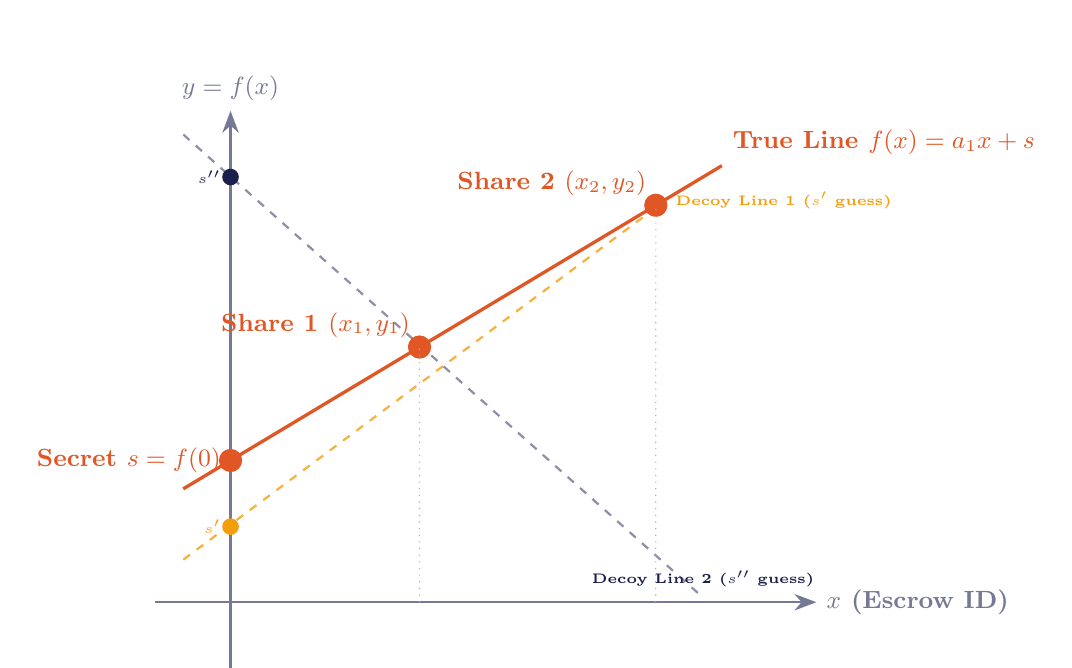
\begin{tikzpicture}[scale=1.2]
		% Axes
		\draw[-{Stealth[scale=1.2]}, thick, color=secondary!60] (-0.8,0) -- (6.2,0) node[right, font=\small\bfseries] {$x$ (Escrow ID)};
		\draw[-{Stealth[scale=1.2]}, thick, color=secondary!60] (0,-0.8) -- (0,5.2) node[above, font=\small\bfseries] {$y = f(x)$};

		% True Secret Intercept S = f(0)
		\fill[color=primary] (0, 1.5) circle (3.5pt) node[left, font=\small\bfseries, color=primary] {Secret $s = f(0)$};

		% Coordinates
		\coordinate (P1) at (2.0, 2.7);
		\coordinate (P2) at (4.5, 4.2);

		% Decoy Lines through P1 with different Y-intercepts
		\draw[dashed, color=accent!80, thick] (-0.5, 0.45) -- (4.6, 4.25) node[right, font=\tiny\bfseries, color=accent] {Decoy Line 1 ($s'$ guess)};
		\draw[dashed, color=secondary!50, thick] (-0.5, 4.95) -- (5.0, 0.05) node[above, font=\tiny\bfseries, color=secondary] {Decoy Line 2 ($s''$ guess)};
		\fill[color=accent] (0, 0.8) circle (2.5pt) node[left, font=\tiny\bfseries, color=accent] {$s'$};
		\fill[color=secondary] (0, 4.5) circle (2.5pt) node[left, font=\tiny\bfseries, color=secondary] {$s''$};

		% True Unique Secret Line
		\draw[very thick, color=primary] (-0.5, 1.2) -- (5.2, 4.62) node[above right, font=\small\bfseries, color=primary] {True Line $f(x) = a_1 x + s$};

		% Escrow Shares
		\fill[color=primary] (P1) circle (3.5pt) node[above left, font=\small\bfseries, color=primary] {Share 1 $(x_1, y_1)$};
		\draw[dotted, color=primary!60] (2.0, 0) -- (P1);

		\fill[color=primary] (P2) circle (3.5pt) node[above left, font=\small\bfseries, color=primary] {Share 2 $(x_2, y_2)$};
		\draw[dotted, color=primary!60] (4.5, 0) -- (P2);

	\end{tikzpicture}%
	}
	\caption{Geometric Intuition of Threshold Secret Sharing: 1 share $(x_1, y_1)$ permits infinitely many candidate lines (dashed), whereas 2 shares $(x_1, y_1)$ and $(x_2, y_2)$ uniquely lock the secret intercept $s = f(0)$.}
	\label{fig:line_principle}
\end{figure}

\subsubsection{Lagrange Coefficients \& Exponentiation Homomorphism}
Given a subset $S \subseteq \{1, \dots, n\}$ of $t$ participating escrow nodes, the Lagrange basis polynomial $L_i(x)$ for participant $i \in S$ is defined as:
\[
	L_i(x) = \prod_{j \in S, j \ne i} \frac{x - x_j}{x_i - x_j}
\]
Notice that $L_i(x_i) = 1$, and $L_i(x_j) = 0$ for all $j \ne i$. Evaluating at $x = 0$ yields the \textbf{Lagrange coefficient} $\lambda_i$:
\[
	\lambda_i = L_i(0) = \prod_{j \in S, j \ne i} \frac{-x_j}{x_i - x_j} \pmod q
\]
The secret exponent $s = f(0)$ is a linear combination of secret shares $z_i$:
\[
	s = \sum_{i \in S} z_i \cdot \lambda_i \pmod q
\]

In ElGamal threshold decryption, the escrow nodes do \textbf{not} reveal their private shares $z_i$. Instead, each escrow node $i$ submits a partial decryption $d_i = a^{z_i} \bmod P$. The requesting node combines these partials in the exponent using Lagrange coefficients:
\[
	a^s = a^{\sum_{i \in S} z_i \cdot \lambda_i} = \prod_{i \in S} \left( a^{z_i} \right)^{\lambda_i} = \prod_{i \in S} d_i^{\lambda_i} \pmod P
\]
The group secret $m$ is then extracted without revealing $s$ or any individual share $z_i$:
\[
	m = b \cdot (a^s)^{-1} \bmod P
\]

% =============================================================================
% 4. SPECIALLY INTERESTING & HARD FUNCTIONS
% =============================================================================
\section{Function Deep Dives: Complex \& Critical Algorithms}
\label{sec:hard_functions}

This section highlights the implementation details of the most mathematically and architecturally non-trivial functions in the project.

% -----------------------------------------------------------------------------
\subsection{Chaum-Pedersen ZKP Generation \& Verification}
Located in \texttt{src/pkg/vote.cxx}, \texttt{VoteClient::PartialDecrypt} and \texttt{VerifyPartialDecryptZKP} prove that an escrow node correctly used its share $z_i$ without leaking it.

\begin{lstlisting}[caption={Chaum-Pedersen ZKP Generation in \texttt{VoteClient::PartialDecrypt}}]
std::pair<PartialDecryption_Struct, DecryptionZKP_Struct>
VoteClient::PartialDecrypt(ElGamal_Ciphertext ciphertext,
                           CryptoPP::Integer partial_pk,
                           CryptoPP::Integer sk) {
  CryptoPP::AutoSeededRandomPool prng;
  CryptoPP::Integer r(prng, CryptoPP::Integer::One(), DL_Q - 1);

  PartialDecryption_Struct pd_s;
  pd_s.d = CryptoPP::ModularExponentiation(ciphertext.a, sk, DL_P);
  pd_s.aggregate_ciphertext = ciphertext;

  DecryptionZKP_Struct dz_s;
  dz_s.u = CryptoPP::ModularExponentiation(DL_G, r, DL_P);
  dz_s.v = CryptoPP::ModularExponentiation(ciphertext.a, r, DL_P);

  CryptoPP::Integer sigma = hash_dec_zkp(partial_pk, ciphertext.a, pd_s.d, dz_s.u, dz_s.v) % DL_Q;
  CryptoPP::Integer temp = CryptoPP::ModularMultiplication(sk, sigma, DL_Q);
  dz_s.s = (r + temp) % DL_Q;

  return {pd_s, dz_s};
}
\end{lstlisting}

\begin{infobox}[ZKP Verification Insight]
	The verification step in \texttt{VerifyPartialDecryptZKP} checks both equations in parallel:
	\[
		G^s \stackrel{?}{=} u \cdot (pk_i)^\sigma \pmod P \quad \text{and} \quad a^s \stackrel{?}{=} v \cdot (d_i)^\sigma \pmod P
	\]
	If both hold, the requester accepts that $d_i$ is consistent with the supplied public share under the implemented Fiat--Shamir-style check. The check is described by the equations above, but its transcript encoding in \texttt{hash\_dec\_zkp} concatenates variable-length decimal integers without length prefixes or domain separation; this is not a canonical production NIZK encoding.
\end{infobox}

% -----------------------------------------------------------------------------
\subsection{Threshold Secret Combination with Lagrange Interpolation}
Located in \texttt{src/pkg/vote.cxx}, \texttt{VoteClient::CombineResults} combines $t$ verified partial decryptions to extract the group key.

\begin{lstlisting}[caption={Lagrange Combination in \texttt{VoteClient::CombineResults}}]
CryptoPP::Integer VoteClient::CombineResults(
    ElGamal_Ciphertext ciphertext,
    std::vector<Escrow_PartialDecryption_Message> all_partial_decryptions) {

  CryptoPP::Integer combined_d = CryptoPP::Integer::One();
  CryptoDriver crypto_driver;

  std::vector<int> participants;
  for (const auto& msg : all_partial_decryptions) {
    participants.push_back(std::stoi(msg.escrow_id));
  }

  for (size_t i = 0; i < all_partial_decryptions.size(); i++) {
    int participant_idx = std::stoi(all_partial_decryptions[i].escrow_id);
    CryptoPP::Integer lambda_i = crypto_driver.ComputeLagrangeCoeff(participant_idx, participants);

    CryptoPP::Integer d_i = all_partial_decryptions[i].dec.d;
    CryptoPP::Integer d_i_pow_lambda = CryptoPP::ModularExponentiation(d_i, lambda_i, DL_P);
    combined_d = CryptoPP::ModularMultiplication(combined_d, d_i_pow_lambda, DL_P);
  }

  CryptoPP::Integer inv_c1_sk = CryptoPP::EuclideanMultiplicativeInverse(combined_d, DL_P);
  CryptoPP::Integer m = CryptoPP::ModularMultiplication(ciphertext.b, inv_c1_sk, DL_P);
  return m;
}
\end{lstlisting}

% -----------------------------------------------------------------------------
\medskip
\subsection{Incremental Group Message Fetching \& State Synchronization}
Located in \texttt{src/pkg/user.cxx} and \texttt{src/drivers/tui/tui\_driver.cpp}, client fetching avoids transferring full message histories repeatedly by tracking an in-memory cursor. The current TUI opens a fresh authenticated connection for each poll; it does not reuse a persistent client session.

\begin{lstlisting}[caption={Incremental Fetch Logic in \texttt{UserClient}}]
// Client sends a since_id cursor on a fresh authenticated connection.
UserToServer_GroupFetch_Message req;
req.group_id = group_id;
req.since_id = this->group_fetch_cursor[key]; // default 0 on start

// Server queries database for new messages only:
// SELECT ... FROM group_message WHERE group_id = ? AND id > ? ORDER BY id ASC;
\end{lstlisting}

% =============================================================================
% 5. SECURITY ANALYSIS & THREAT MODEL
% =============================================================================
\section{Security Analysis \& Threat Model}
\label{sec:security}

\subsection{Threat Model Classification}
\begin{itemize}
	\item \textbf{Server Entity:} Modeled as \textit{Honest-but-Curious}. The server accurately follows protocol steps and forwards messages, but attempts to read plaintexts or reconstruct group keys.
	\item \textbf{Escrow Trustees:} Up to $t-1$ escrows may be maliciously colluding or compromised.
	\item \textbf{Network Attacker:} Passive eavesdropper and active manipulator on client-server channels.
\end{itemize}

\subsection{Security Guarantees}
Table~\ref{tab:security} summarizes the confidentiality, integrity, authorship, and recovery properties provided by the implemented protocol.

\begin{table}[htbp]
	\centering
	\small
	\begin{tabularx}{\textwidth}{l X}
		\toprule
		\textbf{Property} & \textbf{Cryptographic Basis}                                                   \\
		\midrule
		Transport confidentiality & Fresh signed-DH session keys with AES-CBC encrypt-then-HMAC records. \\
		Group confidentiality & AES-CBC under keys derived from the one shared group secret.           \\
		Group integrity and authorship & A group HMAC is checked before decryption; an RSA-PSS signature over the canonical encrypted record authenticates its certified sender. \\
		Setup origin & Creator RSA-PSS signature over the group-creation request and server-certified public keys. \\
		Threshold recovery & $t$-of-$n$ Feldman/ElGamal recovery when the roster is consistent and the escrow secrets remain protected. \\
		Server blindness  & Partial decryptions are encrypted to the requesting escrow under ephemeral DH keys. \\
		\bottomrule
	\end{tabularx}
\caption{Security Guarantees Summary}
\label{tab:security}
\end{table}

% =============================================================================
% 6. BUILD, TESTING & USER INSTRUCTIONS
% =============================================================================
\section{Build System \& Usage Guide}
\label{sec:build}

\subsection{Tested with:}
\begin{itemize}
	\item \textbf{Compiler:} g++ 15.2.1
	\item \textbf{Libraries:} CryptoPP (\texttt{libcrypto++ 8.8.0}), 
	FTXUI (\texttt{v7.0.1}), SQLite3 (\texttt{v3.50.2}), CMake (\texttt{v3.31.11}).
\end{itemize}

From the repository root, run \texttt{mkdir -p build \&\& cd build}, followed by \texttt{cmake ..} and \texttt{make}. The binaries are written to \texttt{build/}.

\end{document}
